\documentclass{beamer}
\usetheme{CambridgeUS}
\title[Process]{The Koopman operator identification algorithm}
\subtitle{So far}
\institute[Polimi]{Politecnico di Milano}
\author{Sergio Vanegas}
\date{\today}

\usepackage{listings}
\usepackage[framed,numbered,autolinebreaks,useliterate]{mcode/mcode}

\usepackage{caption}
\usepackage{subcaption}

\usepackage{siunitx}


\begin{document}

\begin{frame}[plain,noframenumbering]
    \maketitle
\end{frame}


\section{Pre-requisites}

\begin{frame}[fragile]{The forced Van Der Pol oscillator}
    \begin{equation}
        \begin{cases}
            \dot{x}_1 = 2*x_2 \\
            \dot{x}_2 = -0.8*x_1 + 2*x_2 + 10*x_1^2*x_2 + u
        \end{cases}
    \end{equation}

    \begin{lstlisting}[language=Matlab]
function dxdt = VanDerPol(t,x,u_t,u)
    % Interpolation just for the sake of indexing
    u = interp1(u_t,u,t);

    dxdt = [2*x(2);
            -0.8*x(1)+2*x(2)-10*(x(1)^2)*x(2) + u];
end
    \end{lstlisting}
\end{frame}

\begin{frame}{Data generation - Parameters}
    \begin{itemize}
        \item $T_s = \SI{1}{\milli \second}$.
        \item $T = \SI{20}{\second}$.
        \item $N_\text{Sim} = \num{100}$.
        \item $\textbf{u}$: random Gaussian signal with the same sampling rate and length as the simulation.
        \item $\sigma = 1$: std deviation of the Gaussian noise.
        \item $\mu$: average of the Gaussian noise (randomly selected).
    \end{itemize}
\end{frame}

\begin{frame}[fragile]{Data generation - Noise as input}
    \begin{lstlisting}[language=Matlab,basicstyle=\tiny]
Data_Source = "~/Documents/Thesis/VanDerPol_Unsteady_Input/";
ts = 1e-3;
T = 20;
N_Sim = 40;

u_t = 0:ts:T;
sigma = 1; % 0 for constant input
mu = 0;

system("mkdir -p "+Data_Source);
delete(Data_Source+"Data_*.mat");

parfor f=1:N_Sim
    mu = randn(1); % 0 for zero-mean noise
    u = sigma^2*randn(size(u_t)) + mu;
    z0 = 4*rand(2,1) - 2;
    [~,z] = ode113(@(t,z) VanDerPol(t,z,u_t,u), u_t, z0);
    
    z = z';
    L = length(z)-1;
    parsave(sprintf(Data_Source+'Data_%i.mat',f),L,z,u,T,ts);
end
    \end{lstlisting}
\end{frame}

\begin{frame}[fragile]{Polynomial observables}
    \begin{lstlisting}[language=Matlab,basicstyle=\tiny]
function [g,n] = Poly_Obs(z,P,Nx,Nu)
    % Number of monomials with degree lesser than P
    n = factorial(Nx+P)/(factorial(Nx)*factorial(P));
    g = ones(n+Nu,size(z,2));

    exponents = zeros(n,Nx);
    current = zeros(1,Nx);

    [exponents,~] = Recursive_Monomial(1,1,exponents,current,P);

    for i=1:n
        for j=1:Nx
            g(i,:) = g(i,:).*(z(j,:).^exponents(i,j));
        end
    end
    
    % Inputs returned as additional observables
    g(n+1:end,:) = z(Nx+1:end,:);
end
    \end{lstlisting}
\end{frame}

\begin{frame}[fragile]{Recursive exponent generation}
    \begin{lstlisting}[language=Matlab,basicstyle=\tiny]
function [exponents,i] = Recursive_Monomial(i,j,exponents,current,P)
    while sum(current) <= P
        % Decide wether or not to register the exponent combination only on the deepest level of recursion
        if j==size(exponents,2)
            exponents(i,:) = current;
            i = i+1;
        else
            [exponents,i] = Recursive_Monomial(i,j+1,exponents,current,P);
        end

        % Reset exponent count
        current(j) = current(j)+1;
    end
    current(j) = 0;
end
    \end{lstlisting}
\end{frame}


\section{First step: data observables}

\begin{frame}[fragile]{Data reading \& Polynomial degree selection}
    Up to fourth order polynomials used for the presentation (lower order more stable but just as inaccurate).

    \begin{lstlisting}[language=Matlab]
data = dir(Data_Source+"Data_*.mat");
load(Data_Source+data(1).name);

P = 15;
[g_t,n] = Poly_Obs(z,P);

Px = zeros(n,length(data)*L);
Py = Px;
Z = zeros(size(z,1),length(data)*L);
U = zeros(size(u,1),length(data)*L);
    \end{lstlisting}
\end{frame}

\begin{frame}[fragile]{Data concatenation}
    \begin{lstlisting}[language=Matlab]
Px(:,1:L) = g_t(:,1:end-1);
Py(:,1:L) = g_t(:,2:end);
Z(:,1:L) = z(:,1:end-1);
U(:,1:L) = u(:,1:end-1);

for f=2:length(data)
    load(Data_Source+data(f).name);
    [g_t,~] = Poly_Obs(z,P);
    Px(:,L*(f-1)+1:L*f) = g_t(:,1:end-1);
    Py(:,L*(f-1)+1:L*f) = g_t(:,2:end);
    Z(:,L*(f-1)+1:L*f) = z(:,1:end-1);
    U(:,L*(f-1)+1:L*f) = u(:,1:end-1);
end
    \end{lstlisting}
\end{frame}


\section{Second step: operator matrix}

\begin{frame}{Matrix calculation - Notation}
    \begin{itemize}
        \item $\mathbf{u}\left[k\right]$: input vector at sample $k \in \left\{1,\dots,K+1\right\}$.
        \item $\left(\mathbf{x}\left[k\right],\mathbf{y}\left[k\right]\right)$: state pairs such that, for a generic causal DT system $\mathbf{x}\left[k+1\right] = \mathbf{T}(\mathbf{x}\left[k\right] , \mathbf{u}\left[k\right])$, $\mathbf{y}\left[k\right] = \mathbf{T}(\mathbf{x}\left[k\right], \mathbf{u}\left[k\right])$. States are of dimension $N_x$, and the input is of dimension $N_u$.
        \item $P_N$: Projection over the N-Dimensional truncated space of observables, where $\tilde{N} = \frac{\left(N_x + P\right)!}{N_x! P!}$ and $N = \tilde{N} + N_u$.
        \item $p_j$: Monomial observing the original states, with $j \in {1,\dots,\tilde{N}}$.
        \item $\mathbf{P_x},\mathbf{P_y},\mathbf{Z}$: State data collections of the form
            \begin{align*}
                \mathbf{P_x} &= 
                \begin{pmatrix}
                    \mathbf{p}\left(\mathbf{x}\left[1\right]\right)   &
                    \cdots  &
                    \mathbf{p}\left(\mathbf{x}\left[K\right]\right)
                \end{pmatrix}
                \\
                \mathbf{P_y} &= 
                \begin{pmatrix}
                    \mathbf{p}\left(\mathbf{y}\left[1\right]\right)   &
                    \cdots  &
                    \mathbf{p}\left(\mathbf{y}\left[K\right]\right)
                \end{pmatrix}
                \\
                \mathbf{Z} &= 
                \begin{pmatrix}
                    \mathbf{x}\left[1\right]    &
                    \cdots  &
                    \mathbf{x}\left[K\right]
                \end{pmatrix}
            \end{align*}
        \item $\mathbf{U}$: Input data collection of the form $\begin{pmatrix} \mathbf{u}\left[1\right] & \cdots & \mathbf{x}\left[K\right] \end{pmatrix}$.
    \end{itemize}
\end{frame}

\begin{frame}{Matrix calculation - I}

    We denote the associated Koopman operator with sampling time $T_s$ by $\mathcal{K}^{T_s}$, derived from the solution to the following minimization problem:

    \begin{align}
        P_N & g = \text{arg min}_{\tilde{g} \in \text{span}\left\{p_1 , \dots , p_N , u_1 , \dots , u_m\right\}} \sum_{k=1}^K \left|\tilde{g}\left(\mathbf{x}_k\right) - g\left(\mathbf{x}_k\right)\right|^2 \\
        &\implies P_N g =
        \begin{pmatrix}
            g\left(\mathbf{x}_1\right) &
            \cdots &
            g\left(\mathbf{x}_K\right)
        \end{pmatrix}
        \begin{pmatrix}
            \mathbf{P}_x \\
            \mathbf{U}
        \end{pmatrix}^\dagger
        \begin{pmatrix}
            \mathbf{p} \\
            \mathbf{u}
        \end{pmatrix}\\
        & \implies P_N \left(\mathcal{K}^{T_s} p_j\right) = \mathbf{p}^T \mathbf{P_x}^\dagger
        \begin{pmatrix}
            \mathcal{K}^{T_s} p_j\left(\mathbf{x}_1\right) \\
            \vdots \\
            \mathcal{K}^{T_s} p_j\left(\mathbf{x}_K\right)
        \end{pmatrix}
        \approx
        \begin{pmatrix}
            p_j\left(\mathbf{y}_1\right) \\
            \vdots \\
            p_j\left(\mathbf{y}_K\right)
        \end{pmatrix}
        \begin{pmatrix}
            \mathbf{P}_x \\
            \mathbf{U}
        \end{pmatrix}^\dagger
        \begin{pmatrix}
            \mathbf{p} \\
            \mathbf{u}
        \end{pmatrix}
    \end{align}
\end{frame}

\begin{frame}[fragile]{Matrix calculation - II}
    We get each row of the truncation (and, by consequence, the whole matrix) as below, where $A$ and $B$ follow the notation from a classical State Space representation:

    \begin{equation} \label{eq:Matrix_Operator}
        \overline{\mathcal{K}}_{N,j} \approx \mathbf{P}_{y,j} \begin{pmatrix}
            \mathbf{P}_x \\
            \mathbf{U}
        \end{pmatrix}^\dagger \implies \overline{\mathcal{K}}_N = 
        \begin{bmatrix}
            A & B
        \end{bmatrix}
        \approx \mathbf{P}_y
        \begin{pmatrix}
            \mathbf{P}_x \\
            \mathbf{U}
        \end{pmatrix}^\dagger
    \end{equation}
    
    We implement Equation~\ref{eq:Matrix_Operator} as follows:

    \begin{lstlisting}
[A,B] = Koopman(Px,Py,U);
% Generic way to recover original states
C = Unobserver(Px,Z);
% Recovery of original states independent from input
D = zeros(size(Z,1),size(U,1));
save(sprintf(Data_Source+'Operator_P_%i.mat',P), ...
    "A","B","C","D","ts");
    \end{lstlisting}
\end{frame}

\begin{frame}[fragile]{Matrix calculation - III}
    The function \texttt{Koopman} called above is defined as follows:

    \begin{lstlisting}[language=Matlab,basicstyle=\tiny]
function [A,B] = Koopman(X,Y,U)
% Following "Practical Considerations" from Korda-Mezic
G = [X;U]*[X;U]';
V = Y*[X;U]';
A = zeros(size(Y,1),size(X,1));
B = zeros(size(Y,1),size(U,1));

%     Matricial division segmented because of memory limits
%     M0 = V/G;
%     A = M0(:,1:size(X,1));
%     B = M0(:,size(X,1)+1:end);

for i=1:size(Y,1)
    m0 = V(i,:)/G;
    A(i,:) = m0(1:size(X,1));
    B(i,:) = m0(size(X,1)+1:end);
end
    \end{lstlisting}
\end{frame}

\begin{frame}[fragile]{Spectral analysis - Code}
    Originally done for DMD purposes, but it keeps being useful for stability analysis.

    \begin{lstlisting}[language=Matlab]
Lambda = eig(A);
figure(1);
scatter(real(Lambda),imag(Lambda));
hold on;
rectangle('Position', [-1 -1 2 2], 'Curvature', 1);
hold off;
    \end{lstlisting}
\end{frame}

\begin{frame}{Spectral analysis - Results}
    \begin{figure}
        \centering
        \begin{subfigure}[b]{0.45\textwidth}
            \centering
            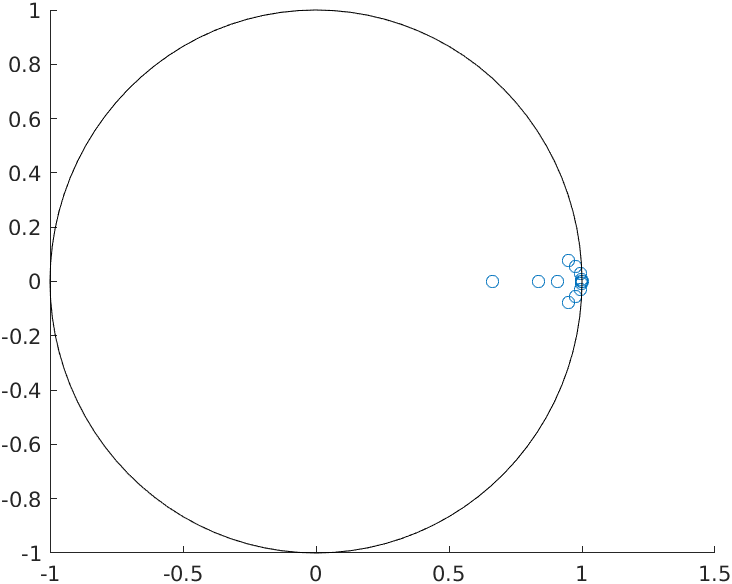
\includegraphics[width=\textwidth]{Steady_Eigen.png}
            \caption{Steady input eigenvalues}
            \label{fig:steady_eigen}
        \end{subfigure}
        \hfill
        \begin{subfigure}[b]{0.45\textwidth}
            \centering
            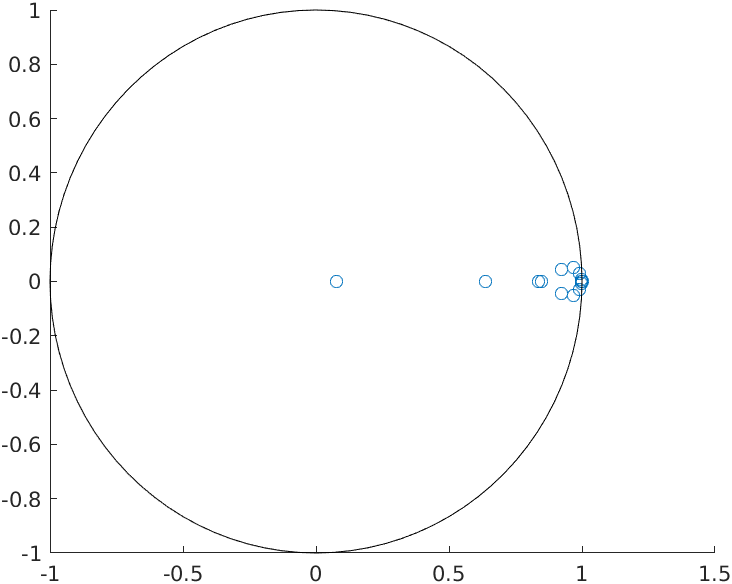
\includegraphics[width=\textwidth]{Unsteady_Eigen.png}
            \caption{Unsteady input eigenvalues}
            \label{fig:unsteady_eigen}
        \end{subfigure}
        \caption{Eigenvalues w.r.t. the Real-Imaginary unit circle}
        \label{fig:eigen}
    \end{figure}
\end{frame}


\section{Trajectory prediction}

\begin{frame}[fragile]{Training data - Visualization}
    \begin{lstlisting}[language=Matlab]
load(Data_Source+data(1).name);
L = length(0:ts:T);

markerDecay = 0.001;
figure(2);
scatter(z(1,:),z(2,:),36*exp(-markerDecay*(0:L-1)));
hold on;
    \end{lstlisting}
\end{frame}

\begin{frame}[fragile]{Training data - Trajectory prediction}
    \begin{lstlisting}[language=Matlab]
g_p = zeros(size(g_t,1),L);
g_p(:,1) = Poly_Obs(z(:,1),P);

for i=1:L-1
    g_p(:,i+1) = A*g_p(:,i) + B*u(:,i);
end

z_p = C*g_p;

scatter(z_p(1,:),z_p(2,:),36*exp(-markerDecay*(0:L-1)));
legend("Original Data","Trajectory Prediction");
hold off;
    \end{lstlisting}
\end{frame}

\begin{frame}{Training data - Results}
    \begin{figure}
        \centering
        \begin{subfigure}[b]{0.45\textwidth}
            \centering
            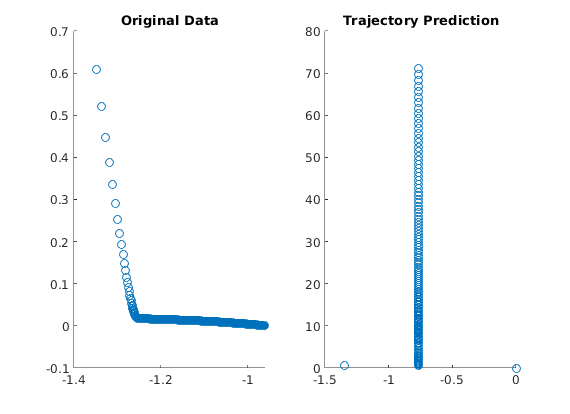
\includegraphics[width=\textwidth]{Steady_Verification.png}
            \caption{Steady input operator verification}
            \label{fig:steady_verify}
        \end{subfigure}
        \hfill
        \begin{subfigure}[b]{0.45\textwidth}
            \centering
            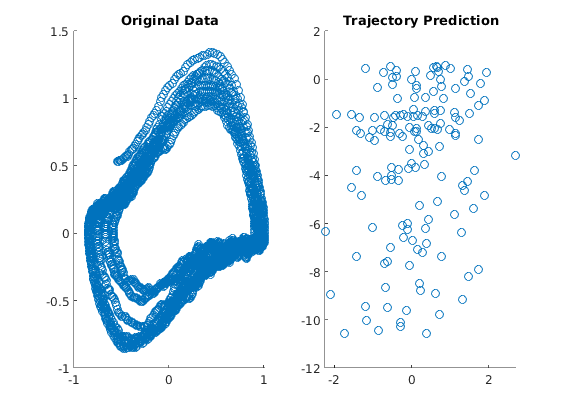
\includegraphics[width=\textwidth]{Unsteady_Verification.png}
            \caption{Unsteady input operator verification}
            \label{fig:unsteady_verify}
        \end{subfigure}
        \caption{Comparison between training trajectory and predicted trajectory}
    \end{figure}
\end{frame}

\begin{frame}[fragile]{New signal - Data generation}
    \begin{lstlisting}[language=matlab]
T = 20;

z0 = 4*rand(2,1) - 2;
sigma = randn(1);
u_t = 0:ts:T;
u = sigma * cos(u_t);

[t,z] = ode113(@(t,z) VanDerPol(t,z,u_t,u), u_t, z0);
z = z';
L = length(0:ts:T);

markerDecay = 0.001;
figure(1);
scatter(z(1,:),z(2,:),36*exp(-markerDecay*(0:L-1)));
hold on;
    \end{lstlisting}
\end{frame}

\begin{frame}[fragile]{New signal - Trajectory prediction}
    \begin{lstlisting}
g_p = zeros(size(g_t,1),L);
g_p(:,1) = Poly_Obs(z(:,1),P);

for i=1:L-1
    g_p(:,i+1) = A*g_p(:,i) + B*u(:,i);
end

z_p = C*g_p;

scatter(z_p(1,:),z_p(2,:),36*exp(-markerDecay*(0:L-1)));
legend("New Simulation","Trajectory Prediction");
hold off;
    \end{lstlisting}
\end{frame}

\begin{frame}{New signal - Results}
    \begin{figure}
        \centering
        \begin{subfigure}[b]{0.45\textwidth}
            \centering
            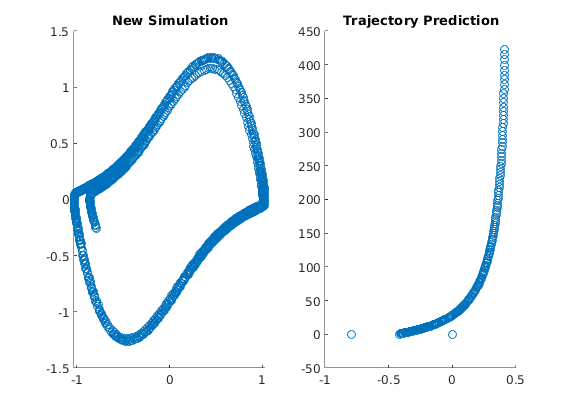
\includegraphics[width=\textwidth]{Steady_NewData.png}
            \caption{Steady input-trained new trajectory prediction}
            \label{fig:steady_new}
        \end{subfigure}
        \hfill
        \begin{subfigure}[b]{0.45\textwidth}
            \centering
            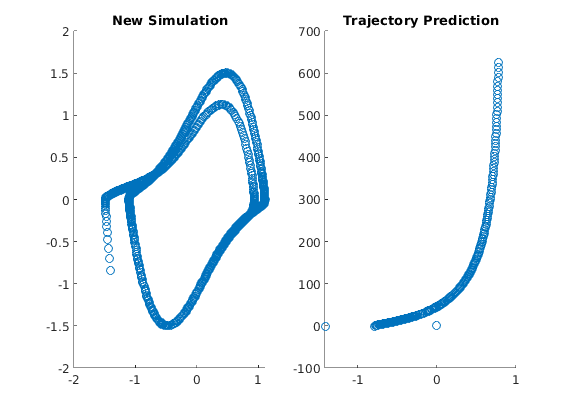
\includegraphics[width=\textwidth]{Unsteady_NewData.png}
            \caption{Unsteady input-trained new trajectory prediction}
            \label{fig:unsteady_new}
        \end{subfigure}
        \caption{Deterministic trajectory prediction test}
    \end{figure}
\end{frame}


\section{Conclusions}

\begin{frame}{Conclusions}
    \begin{itemize}
        \item Lower sampling periods have shown to yield a better prediction horizon, since in practice it is bounded by the variations in shape between different trajectories getting wider throughout physical time.
        \item A classical optimization approach was implemented as part of the development process; nevertheless, it did not produce different results from the pseudo-inverse approach and instead was not able to keep up with the increase in dimension of the observable space. As a consequence, it was removed.
        \item Finally, higher-degree polynomials yielded better approximations of the original system, but required a higher than theoretical data library in order to converge when applying the pseudo-inverse.
    \end{itemize}
\end{frame}

\end{document}